\RequirePackage{xcolor}
\documentclass[cmpiitalkstyle, 22pt]{cmptalk}
\usepackage[utf8]{inputenc}
\usepackage{amsmath}
\usepackage{amssymb}
\usepackage{mathtools,mathdots}
\usepackage{xcolor}
\usepackage{arydshln}
\usepackage{multirow}

\hypersetup{pdfstartpage=1,
  pdfauthor={Pavel Trutman},
  pdfsubject={Master thesis presentation},
  pdftitle={Semidefinite Programming for Geometric Problems in Computer Vision},
  pdfcreator={Pavel Trutman},
  pdfkeywords={computer vision} {polynomial systems solving} {polynomial optimization} {semidefinite programming} {minimal problems},%,pdfpagemode=FullScreen}%,pdfpagemode=None}
  linkcolor={black},
}

\usepackage{bigfig,thumbpdf}
\usepackage[coloremph,display]{texpower}
%\usepackage{movie15}
\usepackage{media9}

\newdimen\tmpd
\newbox\cmptalkverbbox

% notes customization (this one should be before begin document)
\cmptalkeverynotes={\usepackage{multicol}\usepackage{hyperref}\usepackage{movie15}}

\graphicspath{{../images/}{../drawings/}{../}}

\usepackage{enumitem}
\setitemize[1]{leftmargin=2em}
\setitemize[0]{leftmargin=1em}
\setitemize{itemsep=0.2cm,topsep=0.2cm,parsep=0.2cm,partopsep=0pt}
\setenumerate{noitemsep,topsep=0.2cm,parsep=0.2cm,partopsep=0pt,leftmargin=2em}

\newcommand{\bmdB}[1]{\left[\arraycolsep=\arraycolsepdef\begin{array}{@{}#1@{}}}
\newcommand{\bmdE}{\end{array}\right]}
\newcommand{\ind}[1]{\ensuremath{_{#1}}}
\newcommand{\R}{\mathbb{R}}
\newcommand{\N}{\mathbb{N}}
\newcommand{\C}{\mathbb{C}}
\newcommand{\Z}{\mathbb{Z}}
\DeclareMathOperator{\vc}{vec}
\DeclareMathOperator{\tr}{tr}
\newlength{\arraycolsepdef}
\setlength{\arraycolsepdef}{\arraycolsep}

%------------------------------------------------------------------- Title page
%-- specifications
\author{Pavel Trutman}
\affiliation{Centrum strojového vnímání}
\title{Semidefinitní programování v geometrii počítačového vidění}
\acknowledgement{Vedoucí práce: Ing.\ Tomáš Pajdla, Ph.D.\\
Oponent: doc.\ Dr.\ Ing.\ Radim Šára}
\talklogo{
\includegraphics[width=4cm]{cmp}}

\begin{document}
\fontsize{22pt}{26.4pt}\selectfont
\bigfigfalse
\begin{talktitlepage}
  {\fontsize{26pt}{31.2pt}\selectfont
  \mbox{}\\
  {\LARGE\bfseries \thetitle }\\[\baselineskip]
  \theauthor \\[\baselineskip]
  \textit{Vedoucí práce: Ing.\ Tomáš Pajdla, Ph.D.}
  \vfill
  \thetalklogo\\[1cm]
  Centrum strojového vnímání\\
  Katedra kybernetiky\\
  Fakulta elektrotechnická\\
  České vysoké učení technické v Praze
  \vspace{2cm}
  }
\end{talktitlepage}

% --------------------------------------------------------------------------- 
\begin{cmptalkslide}[Obsah]
  \begin{itemize}
    \item Motivace
    \item Metoda momentů a Lasserrova hierarchie
    \item Implementace
    \item Experimenty
    \begin{itemize}
      \item Poloha a orientace kalibrované kamery (P3P)
      \item Poloha a orientace kalibrované kamery s neznámou ohniskovou vzdáleností (P3.5Pf)
    \end{itemize}
    \item Přínosy práce
  \end{itemize}
\end{cmptalkslide}

% --------------------------------------------------------------------------- 
\begin{cmptalkslide}[Motivace]
  \begin{itemize}
    \item Mnoho problémů v geometrii počítačového vidění vede na řešení soustav polynomiálních rovnic
    \item Tyto soustavy umíme řešit algebraicky (Algoritmus $F_4$ \cite{F4}, Automatický generátor \cite{AutoGen})
    \begin{itemize}
      \item jsou vypočtena všechna komplexní řešení, nereálná jsou poté vyřazena
      \item nevhodné na přeurčené soustavy na datech se šumem
    \end{itemize}
    \item Aplikace metod z polynomiální optimalizace řeší tyto problémy
    \begin{itemize}
      \item umíme najít pouze reálná řešení
      \item do systému lze přidat polynomiální nerovnice
      \item lze optimalizovat kriteriální polynomialní funkci na prostoru řešení
    \end{itemize}
  \end{itemize}

  \placeat{
    \Put(0,0.035)[lb]{\footnotesize \cite{F4} J.-C.\ Faugère. A new efficient algorithm for computing gröbner bases ($f_4$).}
    \Put(0,0)[lb]{\footnotesize \cite{AutoGen} Z. Kukelova, M. Bujnak, T. Pajdla. Automatic generator of minimal problem solvers.}
  }

\end{cmptalkslide}


% --------------------------------------------------------------------------- 
\begin{cmptalkslide}[Metoda momentů \cite{MomentMethodReal}]
  \setlength{\abovedisplayskip}{0.9em}
  \setlength{\belowdisplayskip}{0.9em}
  \placeat{
    \Put(0,0.035)[lb]{\footnotesize \cite{Lasserre} J. B. Lasserre. Global optimization with polynomials and the problem of moments.}
    \Put(0,0)[lb]{\footnotesize \cite{MomentMethodReal} J. B. Lasserre, M. Laurent, and P. Rostalski. Semidefinite characterization and computation of zero-dimensional real radical ideals.}
  }

  \begin{itemize}
    \item Založena na Lasserrově hierarchii \cite{Lasserre}
    \item Problém polynomiální optimalizace (nekonvexní)
    \vspace{-0.6em}
    \begin{align}
      \arraycolsep=1.4pt
      \begin{array}{rclrcl@{\hskip0.5cm}l}
        p^* &=& \displaystyle \min_{x\in\R^n} & \multicolumn{3}{l}{f(x)} \\
        && \text{s.t.} & g_i(x) &\geq& 0 & (i = 1,\ldots,k) \\
        &&& h_j(x) &=& 0 & (j = 1,\ldots,l)
      \end{array}
    \end{align}

    \vspace{-1em}
    \item Každý monom nahradíme novou proměnnou: $\ell_y(x^\alpha)=y_\alpha$

    \stepwise{
      \switch{
        \item Semidefinitní problém nekonečné dimenze (konvexní)
        \vspace{-0.6em}
        \begin{align}
          \arraycolsep=1.4pt
          \begin{array}{rclrcl@{\hskip0.5cm}l}
            p^* &=& \displaystyle \min_{y\in\R^{\N^n}} & \multicolumn{3}{l}{\vc(f)^\top y} \\
            && \text{s.t.} & y_{0\ldots0} &=& 1\\
            &&& M(y) &\succeq& 0\\
            &&& M(g_iy) &\succeq& 0 & (i = 1,\ldots,k)\\
            &&& \vc(h)^\top y &=& 0 & \forall h\in \left<h_1,\ldots,h_l\right>
          \end{array}
        \end{align}
      }
      {\stepcounter{equation}
        \item Semidefinitní problém dimenze $\color{cmporange} \binom{n + 2r}{n}$ {\color{cmporange} pro stupeň relaxace $r\in\N$}
        \vspace{-0.6em}
        \begin{align}
          \arraycolsep=1.4pt
          \begin{array}{rclrcl@{\hskip0.5cm}l}
            p^*_{\color{cmporange} r} &=& \displaystyle \min_{y\in\R^{\N^n_{\color{cmporange} 2r}}} & \multicolumn{3}{l}{\vc(f)^\top y} \\
            && \text{s.t.} & y_{0\ldots0} &=& 1\\
            &&& M_{\color{cmporange} r}(y) &\succeq& 0\\
            &&& M_{\color{cmporange} r - \big\lceil\frac{\deg(g_i)}{2} \big\rceil}(g_iy) &\succeq& 0 & (i = 1,\ldots,k)\\
            &&& \vc(h)^\top y &=& 0 & \forall h\in {\color{cmporange} \big\{h_jx^\alpha \ |\ j=1,\ldots,l, |\alpha|\leq2r-\deg(h_j)\big\}}
          \end{array}
        \end{align}
        \vspace{-1em}
        \item Konvergence zajištěna
        \vspace{-0.6em}
        \begin{align}
          p^*_r &\leq p^*_{r+1} \leq p^* & \lim_{r\rightarrow+\infty}p^*_r &= p^*
        \end{align}
      }
    }

  \end{itemize}
  \placeat{
    \Put(0,0.035)[lb]{\footnotesize \cite{Lasserre} J. B. Lasserre. Global optimization with polynomials and the problem of moments.}
    \Put(0,0)[lb]{\footnotesize \cite{MomentMethodReal} J. B. Lasserre, M. Laurent, and P. Rostalski. Semidefinite characterization and computation of zero-dimensional real radical ideals.}
  }


\end{cmptalkslide}

% --------------------------------------------------------------------------- 
%\begin{cmptalkslide}[Metoda momentů \cite{MomentMethodReal}]
  %\begin{itemize}
    %\item Řešíme relaxované SDP pro rostoucí relaxační stupeň $r$
    %\item Existuje test, zda je daná relaxace těsná
    %\item Výpočet řešení přes vlastní vektory multiplikativní matice
  %\end{itemize}

  %\placeat{
    %\Put(.5,0.35){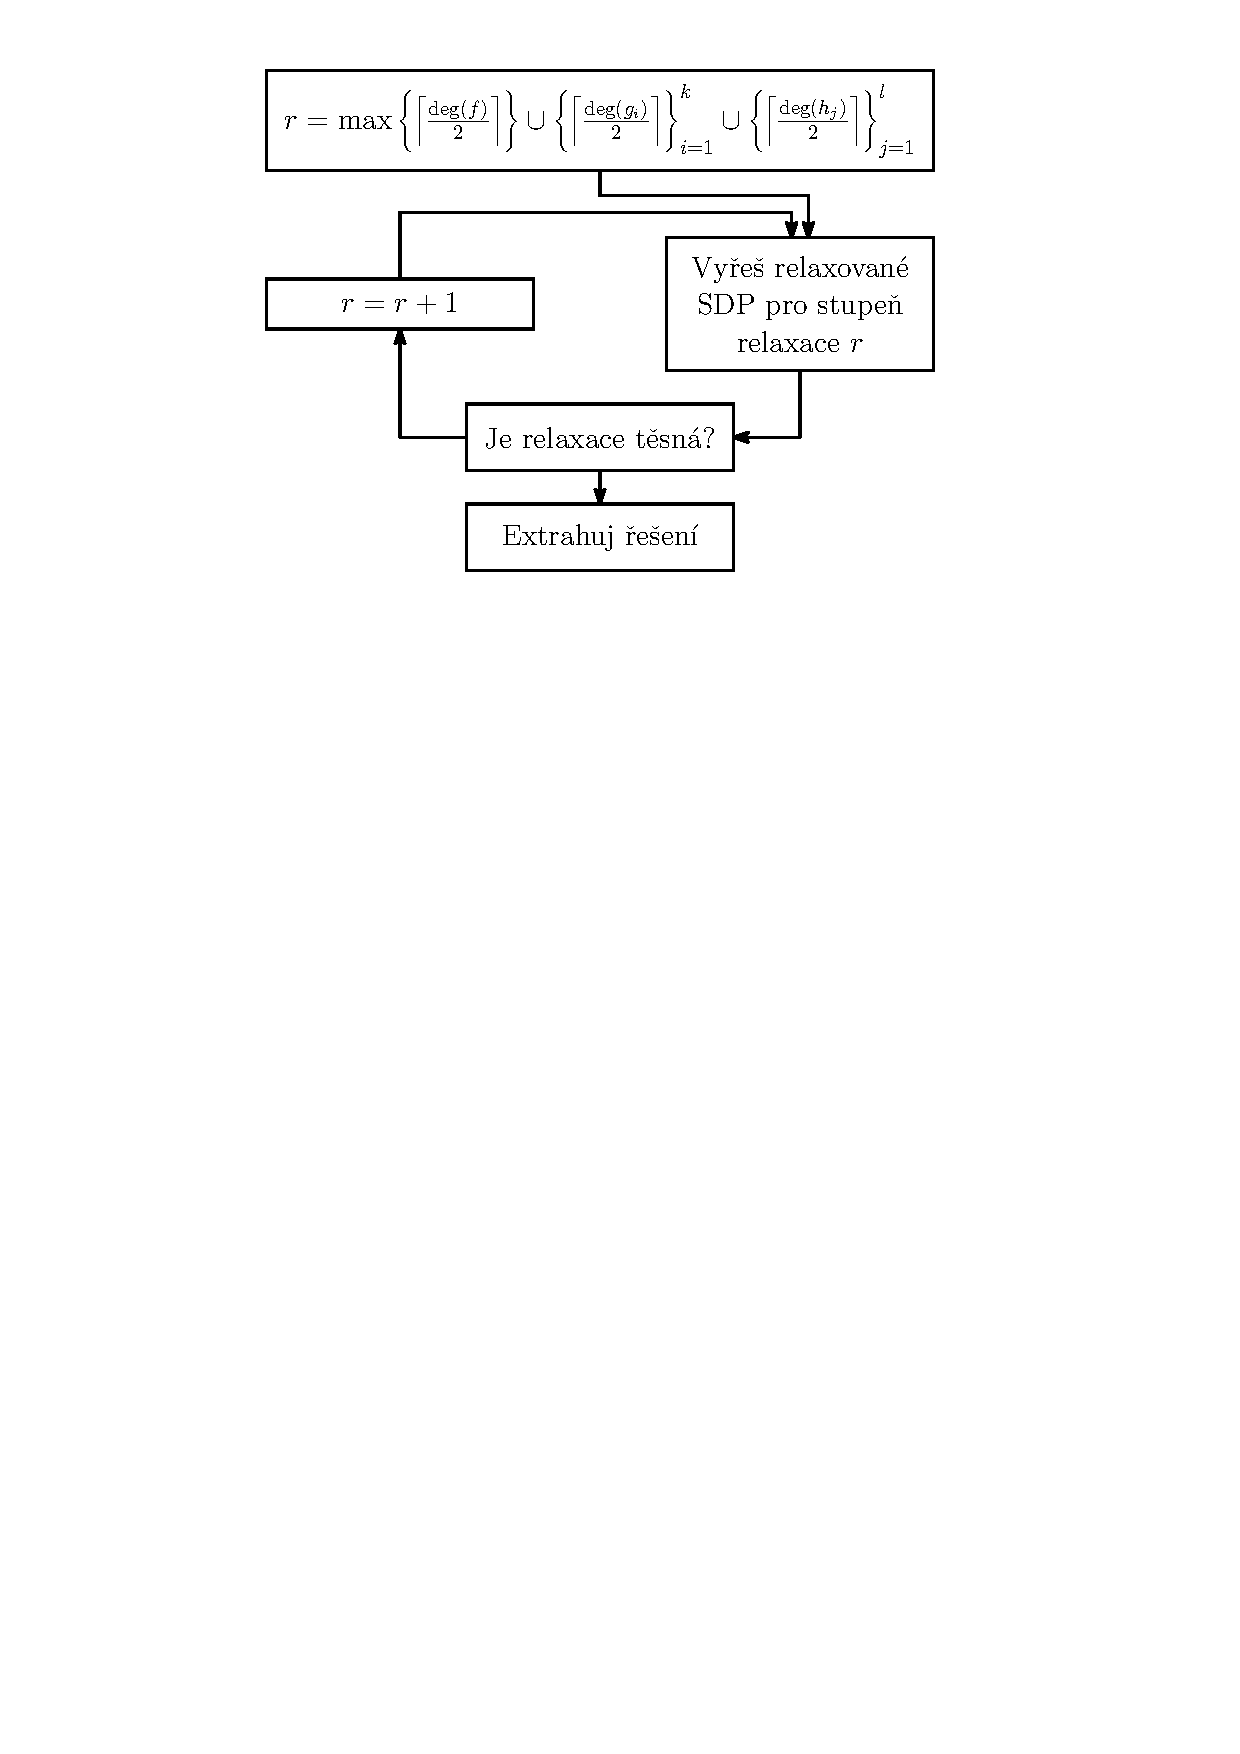
\includegraphics[width=17cm]{pre_momentMethod}}
    %\Put(0,0)[lb]{\footnotesize \cite{MomentMethodReal} J. B. Lasserre, M. Laurent, and P. Rostalski. Semidefinite characterization and computation of zero-dimensional real radical ideals.}
  %}

%\end{cmptalkslide}

% --------------------------------------------------------------------------- 
\begin{cmptalkslide}[Implementace]
  \begin{itemize}
    \item Balíček Polyopt
    \begin{itemize}
      \item programovací jazyk Python
      \item implementace momentové metody
      \item implementace vlastního nástroje na řešení semidefinitních problémů: algoritmus vnitřních bodů s využitím bariérové funkce, dle \cite{Nesterov-2004}
    \end{itemize}
    \item Implementace momentové metody v MATLABu
    \begin{itemize}
      \item využití nastoje MOSEK \cite{mosek} na řešení semidefinitních problémů
      \item využití toolboxu YALMIP \cite{Yalmip} jako interface
    \end{itemize}
  \end{itemize}

  \placeat{
    \Put(0,0.070)[lb]{\footnotesize \cite{Yalmip} Johan L\"{o}fberg. YALMIP: A toolbox for modeling and optimization in MATLAB.}
    \Put(0,0.035)[lb]{\footnotesize \cite{mosek} MOSEK ApS. The MOSEK optimization toolbox for MATLAB manual. Version 7.1 (Revision 28).}
    \Put(0,0)[lb]{\footnotesize \cite{Nesterov-2004} Y. Nesterov. Introductory lectures on convex optimization: A basic course.}
  }

\end{cmptalkslide}

% --------------------------------------------------------------------------- 
\begin{cmptalkslide}[Experimenty]
  \begin{itemize}
    \item Řešení soustav polynomiálních rovnic
    \item Aplikace na minimálních problémech z geometrie počítačového vidění
    \begin{itemize}
      \item Poloha a orientace kalibrované kamery (P3P)
      \item Poloha a orientace kalibrované kamery s neznámou ohniskovou vzdáleností (P3.5Pf)
    \end{itemize}
    \item Testování na reálné 3D scéně
    \begin{itemize}
      \item robustně zrekonstruovaná
      \item 67 kamer, 145\,001 bodů v prostoru
    \end{itemize}
    \item Porovnání různých implementací
    \begin{itemize}
      \item čistě algebraické řešení vygenerované Automatickým generátorem \cite{AutoGen}
      \item balíček Polyopt
      \item implementace v MATLABu s využitím nástroje MOSEK \cite{mosek}
      \item optimalizační nástroj Gloptipoly \cite{gloptipoly}
    \end{itemize}
  \end{itemize}

  \placeat{
    \Put(0.85,0.48){\scalebox{-1}[1]{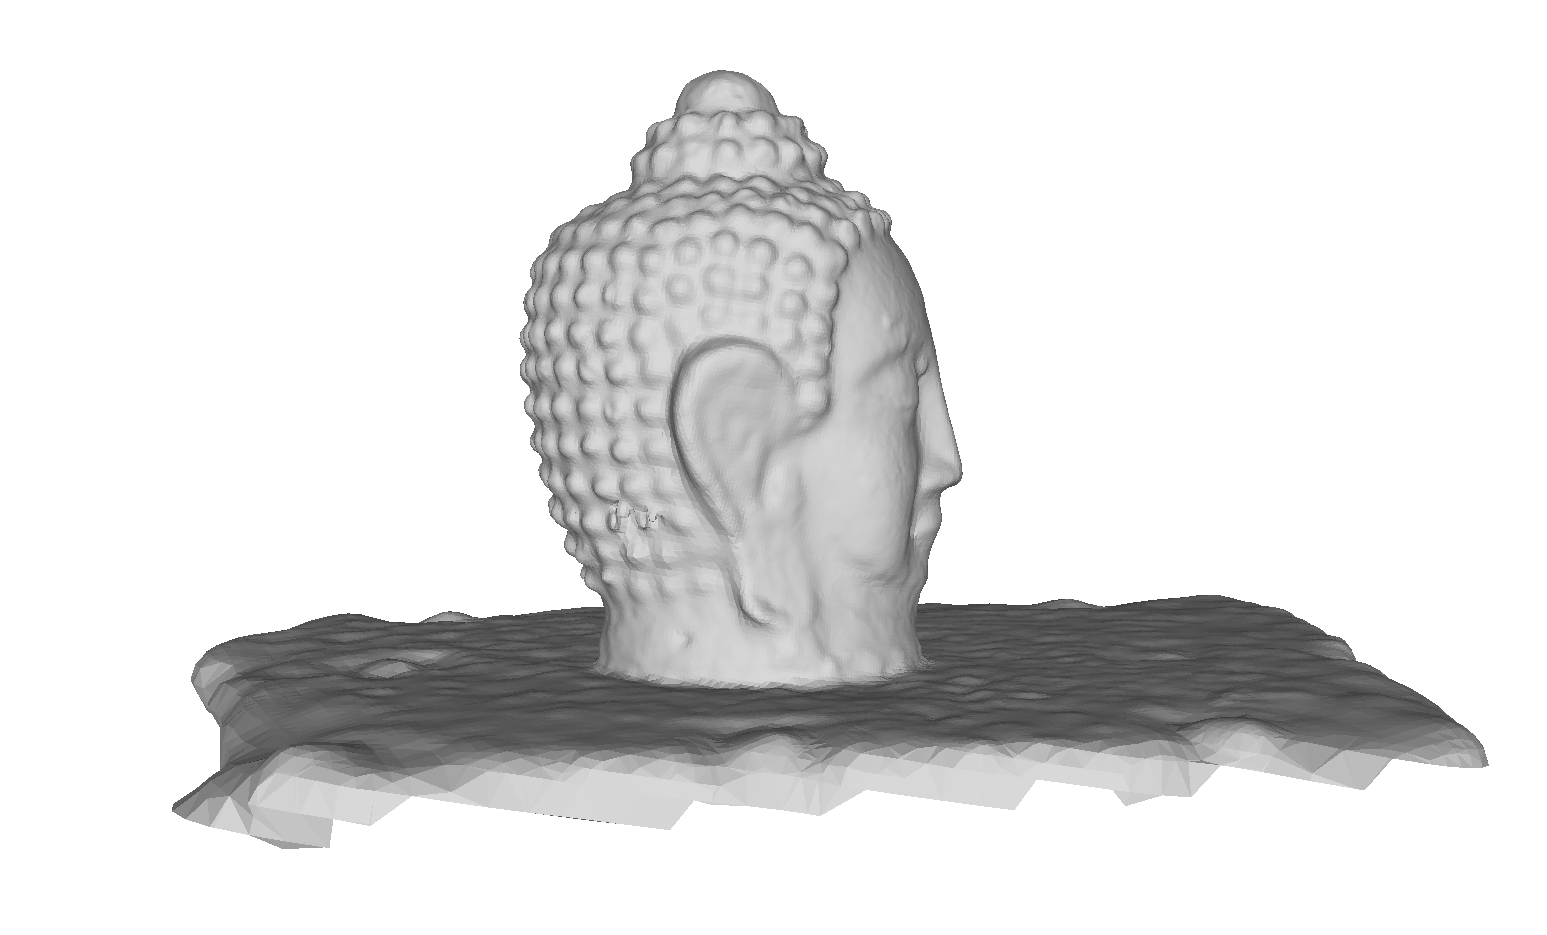
\includegraphics[height=5cm]{LADIO_01}}}
    \Put(0.60,0.48){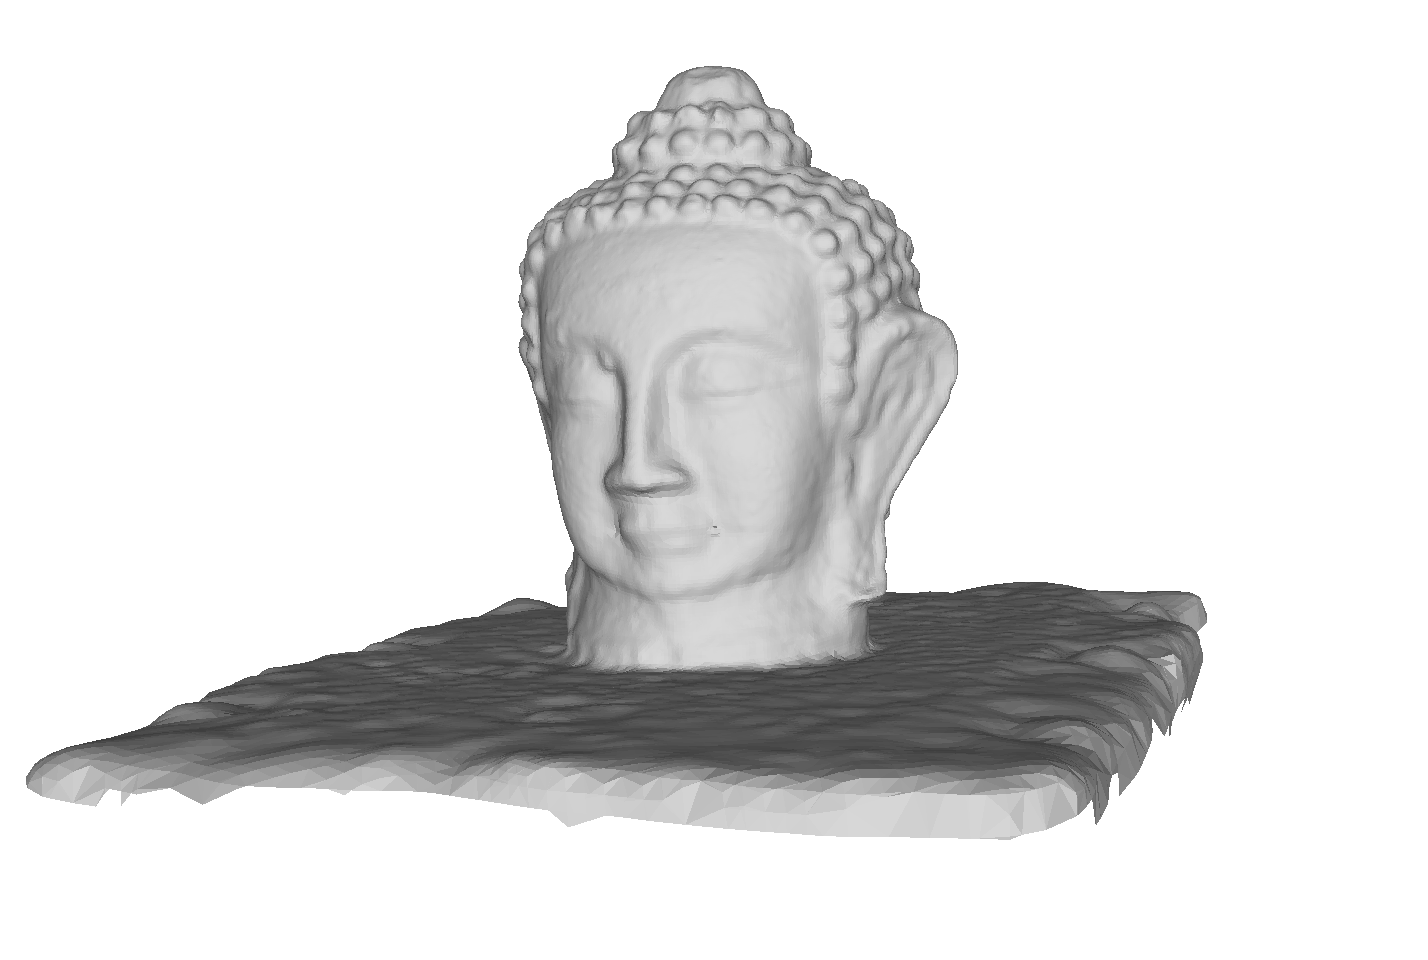
\includegraphics[height=5cm]{LADIO_02}}
    \Put(0,0.070)[lb]{\footnotesize \cite{gloptipoly} D. Henrion, J. B. Lasserre, and J. Löfberg. Gloptipoly 3: Moments, optimization and semidefinite programming.}
    \Put(0,0.035)[lb]{\footnotesize \cite{AutoGen} Z. Kukelova, M. Bujnak, T. Pajdla. Automatic generator of minimal problem solvers.}
    \Put(0,0.000)[lb]{\footnotesize \cite{mosek} MOSEK ApS. The MOSEK optimization toolbox for MATLAB manual. Version 7.1 (Revision 28).}
  }

\end{cmptalkslide}

% --------------------------------------------------------------------------- 
\begin{cmptalkslide}[Poloha a orientace kalibrované kamery (P3P)]
  \begin{minipage}{0.45\textwidth}
    \begin{itemize}
      \item Jedna rovnice čtvrtého stupně
      \item Jedna neznámá
      \item Vybrán nejlepší výsledek z 1000 různých konfigurací pro každou z~67 kamer (RANSAC-like)
      \item 60 \% řešení je reálných
    \end{itemize}
  \end{minipage}

  \placeat{
    \Put(.25,0.05)[cb]{\hyperlink{P3P_err}{\resizebox{0.5\textwidth}{!}{\fontsize{15pt}{18.0pt}\selectfont \input{../graphs/pre_P3P_err}}}}
    \Put(.75,0.05)[cb]{\hyperlink{P3P_times}{\resizebox{0.5\textwidth}{!}{\fontsize{15pt}{18.0pt}\selectfont \input{../graphs/pre_P3P_times}}}}
    \Put(.75,0.45)[cb]{\hyperlink{P3P_relax}{\resizebox{0.5\textwidth}{!}{\fontsize{15pt}{18.0pt}\selectfont \input{../graphs/pre_P3P_relax}}}}
  }

\end{cmptalkslide}

% --------------------------------------------------------------------------- 
\begin{cmptalkslide}[Poloha a orientace kalibrované kamery s neznámou ohniskovou vzdáleností (P3.5Pf)]
  \begin{minipage}{0.45\textwidth}
    \begin{itemize}
      \item Devět rovnic třetího stupně
      \item Čtyři neznámé
      \item Vybrán nejlepší výsledek z 100 různých konfigurací pro každou z~20 vybraných kamer (RANSAC-like)
      \item 48 \% řešení je reálných
    \end{itemize}
  \end{minipage}

  \placeat{
    \Put(.25,0.05)[cb]{\hyperlink{P35Pf_err}{\resizebox{0.5\textwidth}{!}{\fontsize{15pt}{18.0pt}\selectfont \input{../graphs/pre_P35Pf_err}}}}
    \Put(.75,0.05)[cb]{\hyperlink{P35Pf_times}{\resizebox{0.5\textwidth}{!}{\fontsize{15pt}{18.0pt}\selectfont \input{../graphs/pre_P35Pf_times}}}}
    \Put(.75,0.45)[cb]{\hyperlink{P35Pf_relax}{\resizebox{0.5\textwidth}{!}{\fontsize{15pt}{18.0pt}\selectfont \input{../graphs/pre_P35Pf_relax}}}}
  }

\end{cmptalkslide}

% --------------------------------------------------------------------------- 
\begin{cmptalkslide}[Přínosy práce]
  \begin{itemize}
    \item Metoda momentů
    \begin{itemize}
      \item rozbor a implementace metody v Pythonu a MATLABu
      \item použití metody na problémy z geometrie počítačového vidění
      \item aplikace na úlohy z robotiky: řešení inverzní kinematické úlohy
    \end{itemize}
    \item Nástroj na řešení semidefinitních problémů
    \begin{itemize}
      \item implementace v Pythonu
      \item porozumění typům semidefinitních problémů generovaných Lasserrovou hierarchií
      \item využití implementace v rámci formální verifikace algoritmů v konvexní optimalizaci, D. Henrion, LAAS--CNRS v Toulouse
    \end{itemize}
    \item Srovnání implementace momentové metody se současnými nástroji
    \begin{itemize}
      \item stabilita odpovídá algebraickým metodám
      \item nemůže konkurovat algebraickým metodám v rychlosti
    \end{itemize}
  \end{itemize}

  \placeat{
    \Put(.5,0.06){\Large \textbf{Děkuji za pozornost}}
  }
\end{cmptalkslide}

% --------------------------------------------------------------------------- 
%\begin{cmptalkslide}[Shrnutí]
  %\begin{itemize}
    %\item Implementoval jsem nástroj na řešení semidefinitních problémů v Pythonu
    %\item Implementoval jsem metodu momentů v Pythonu a MATLABu
    %\item Porovnal jsem rychlost a stabilitu se současnými nástroji
    %\begin{itemize}
      %\item stabilita odpovídá algebraickým metodám
      %\item nemůže konkurovat algebraickým metodám v rychlosti
    %\end{itemize}
  %\end{itemize}

  %\placeat{
    %\Put(.5,0.30){\Large \textbf{Děkuji za pozornost}}
  %}

%\end{cmptalkslide}

% --------------------------------------------------------------------------- Bibliography
\begin{cmptalkslide}[Použitá literatura]
  \bibliographystyle{plain}
  {\small \bibliography{../citations}}
\end{cmptalkslide}

% --------------------------------------------------------------------------- 
\maskfoil{P3PParametrization}{

  \centering
  {\large\bfseries Parametrizace P3P problému}\\[1em]
  \begin{minipage}{0.50\textwidth}
    \begin{itemize}
      \item Známe 3D body $X_i$ a jejich projekce $x_i$
      \item Napočítáme vzdálenosti mezi 3D body $d_{ij}$ a kosiny úhlů paprsků $c_{ij}$
      \item Z kosinovy věty dostáváme tři rovnice druhého stupně ve třech neznámých $z_i$
      \begin{align}
        d_{ij}^2 &= z_i^2 + z_j^2 - 2z_iz_jc_{ij}\label{eq:P3P:3}
      \end{align}
      \item Manipulací lze upravit na jednu rovnici čtvrtého stupně v jedné neznámé $\xi$
      \begin{align}
        a_4\xi^4 + a_3\xi^3 + a_2\xi^2 + a_1\xi + a_0 &= 0\label{eq:P3P:1}
      \end{align}
      \item Každý parametr $a_k$ je polynomiální funkcí hodnot $d_{ij}$ a $c_{ij}$
    \end{itemize}
  \end{minipage}\hspace{0.45\textwidth}~\\
  \vspace{-17cm}\hspace{16cm}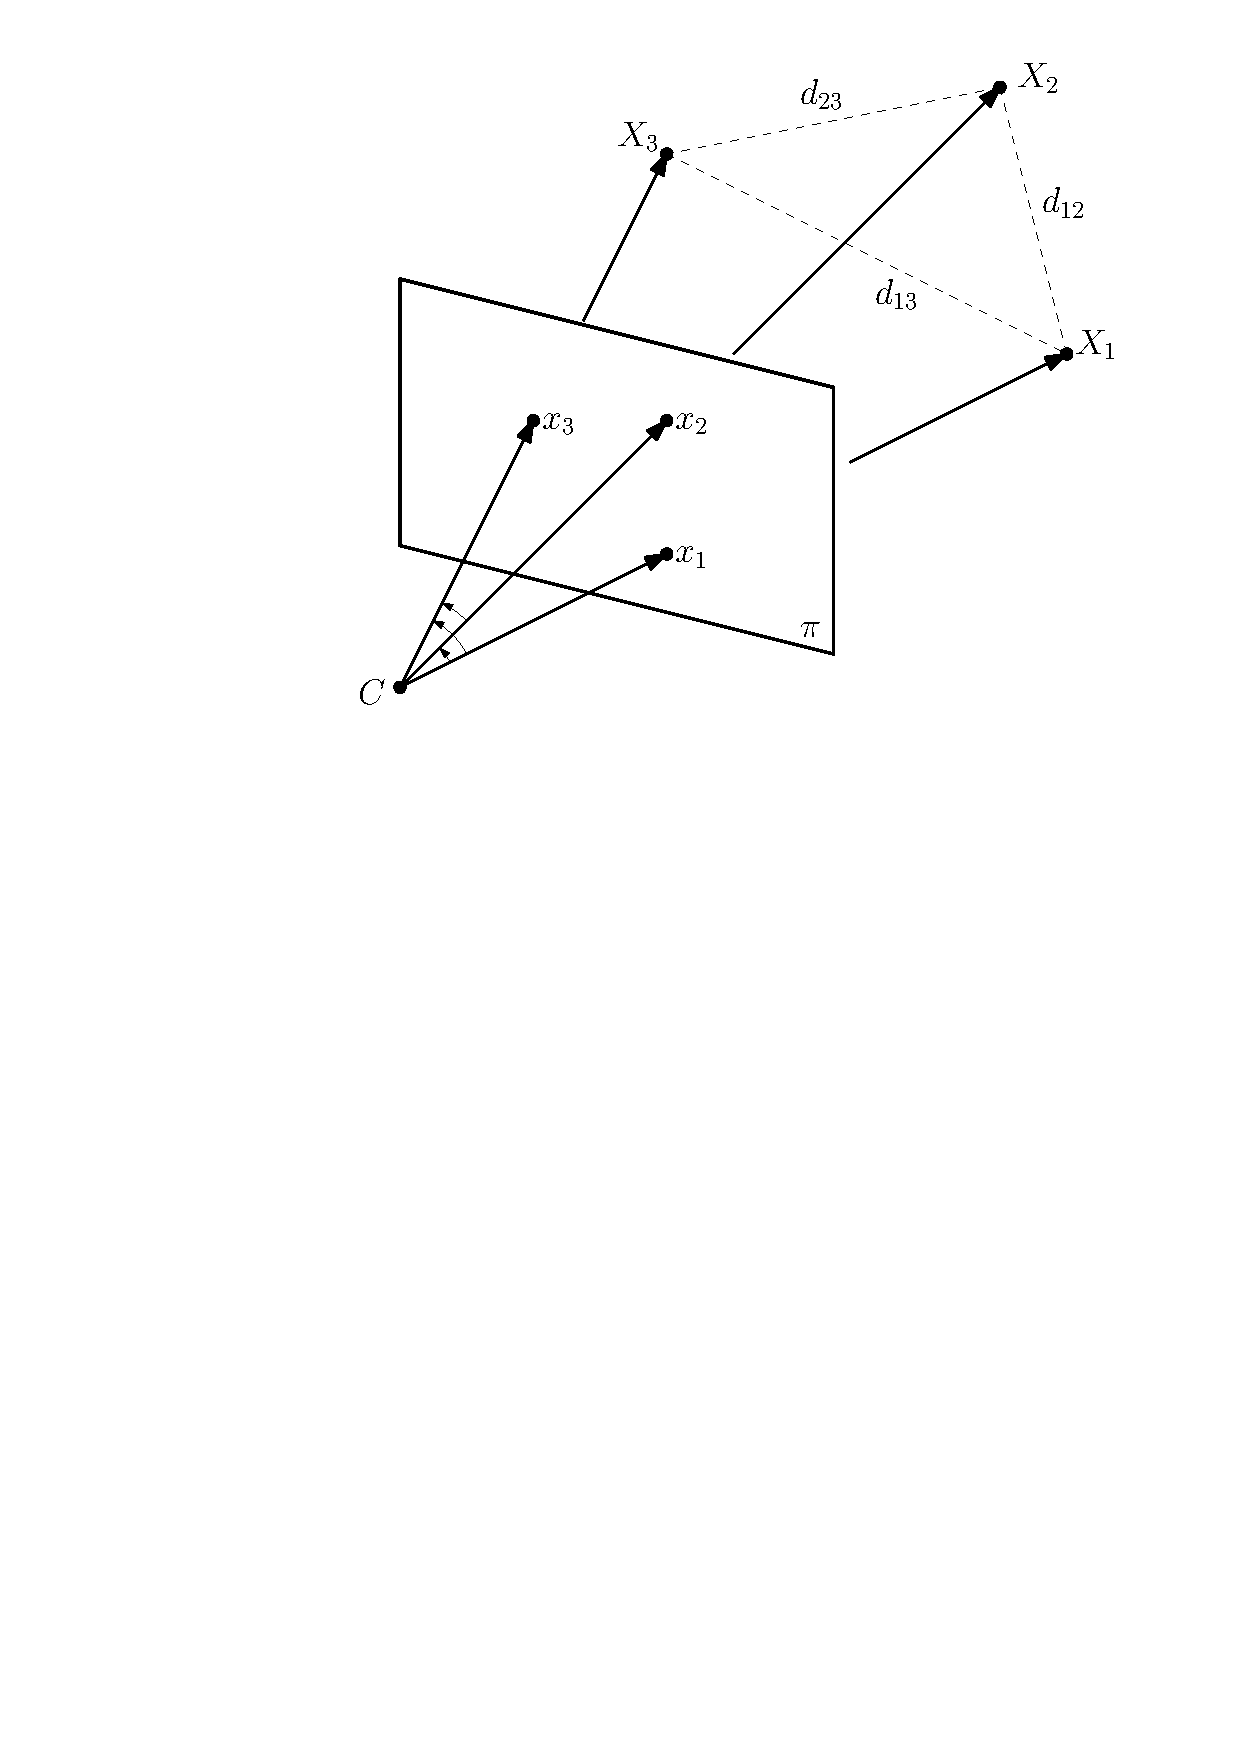
\includegraphics[width=11cm]{drawings/P3P}\\
  \hspace{16cm}\textbf{Obrázek 1. }Nákres P3P problému.\\[2cm]
  \hspace{16cm}\begin{tabular}{|c||c|c|}
    \hline
    $\boldsymbol{r}$ & \textbf{Soustava (\ref{eq:P3P:3})} & \textbf{Soustava (\ref{eq:P3P:1})}\\\hline\hline
    1 & 10 & --\\
    2 & 35 & 5\\
    \textbf{3} & \textbf{84} & \textbf{7}\\\hline
  \end{tabular}\\[5mm]
  \hspace{16cm}\textbf{Tabulka 1. }Počet neznámých řešeného\\
  \hspace{16cm}semidefinitního problému.
}

% --------------------------------------------------------------------------- 
\maskfoil{numberRealSolutions}{

  \centering
  {\large\bfseries Počet nalezených reálných řešení}\\[1em]
  \begin{minipage}{0.95\textwidth}
    \begin{itemize}
      \item Implementace založené na metodě momentů nenaleznou všechna reálná řešení
    \end{itemize}
    \centering
    \vspace{5mm}
    \input{../tables/pre_P3P_numberSolutions.tex}\\[5mm]
    \textbf{Tabulka 1. }Počet nalezených reálných řešení pro P3P problém.\\
    \vspace{1cm}
    \input{../tables/pre_P35Pf_numberSolutions.tex}\\[5mm]
    \textbf{Tabulka 2. }Počet nalezených reálných řešení pro P3.5Pf problém.\\
  \end{minipage}
}

% --------------------------------------------------------------------------- 
\maskfoil{numericalProblems}{

  \centering
  {\large\bfseries Numerické problémy v balíčku Polyopt}\\[1em]
  \begin{minipage}{0.95\textwidth}
    \begin{itemize}
      \item Nástroj na řešení semidefinitních problémů nevyřeší zadaný semidefinitní problém
      \item Metoda založena na minimalizaci bariérové funkce
      \begin{align}
        F(y) &= -\ln\det\!\big(A(y)\big)
      \end{align}
      \item $A(y)$ je semidefinitně pozitivní matice
      \begin{align}
        A(y) &= A_0 + \sum_{k=1}^m A_k y\ind k
      \end{align}
      %\item Optimalizace pomocí upravené Newtonovy metody $\rightarrow$ nutnost vypočítat první a druhé derivace bariérové funkce
      \item Potřeba spočítat první a druhé derivace bariérové funkce
      \begin{align}
        \frac{\partial F}{\partial y\ind i}(y) &= -\tr\!\big(A(y)^{-1}A_i\big)\\
        \frac{\partial^2 F}{\partial y\ind i \partial y\ind j}(y) &= \tr\!\Big(\!\big(A(y)^{-1}A_i\big)\big(A(y)^{-1}A_j\big)\!\Big)
      \end{align}
      \item Použití upravené Newtonovy metody $\rightarrow$ vyčíslení inverze Hessovy matice v bodě
    \end{itemize}
  \end{minipage}
}

% --------------------------------------------------------------------------- 
\maskfoil{momentMatrix}{

  \centering
  {\large\bfseries Momentová matice}\\[1em]
  \begin{minipage}{0.95\textwidth}
    \begin{itemize}
      \item Momentová matice $M(y)$ pro \makebox{$y\in\R^{\N^n}$} má tvar
      \begin{align}
        M(y)\ind{\alpha,\beta}=y_{\alpha+\beta}
      \end{align}
      \item Příklad pro $n=2$:
      \begin{align}
        M(y)&=\bmdB{c:cc:ccc:c}
                y_{00} & y_{10} & y_{01} & y_{20} & y_{11} & y_{02} & \cdots\\\hdashline
                y_{10} & y_{20} & y_{11} & y_{30} & y_{21} & y_{12} & \cdots\\
                y_{01} & y_{11} & y_{02} & y_{21} & y_{12} & y_{03} & \cdots\\\hdashline
                y_{20} & y_{30} & y_{21} & y_{40} & y_{31} & y_{22} & \cdots\\
                y_{11} & y_{21} & y_{12} & y_{31} & y_{22} & y_{13} & \cdots\\
                y_{02} & y_{12} & y_{03} & y_{22} & y_{13} & y_{04} & \cdots\\\hdashline
                \vdots & \vdots & \vdots & \vdots & \vdots & \vdots & \ddots
              \bmdE
      \end{align}
    \end{itemize}
  \end{minipage}
}

% --------------------------------------------------------------------------- 
\maskfoil{localizingMatrix}{

  \centering
  {\large\bfseries Lokalizační matice}\\[1em]
  \begin{minipage}{0.95\textwidth}
    \begin{itemize}
      \item Lokalizační matice $M(qy)$ pro \makebox{$y\in\R^{\N^n}$} a polynom $q(x)$ má tvar
      \begin{align}
        M(qy)\ind{\alpha,\beta}=\sum_{\gamma\in\N^n} q_\gamma y_{\alpha+\beta+\gamma}
      \end{align}
      \item Příklad pro $n=2$ a $q(x) = 5x_1^2 + 8x_2 + 3$:
      \begin{align}
        M(qy)&= 5
        \bmdB{c:cc:c}
          y_{20} & y_{30} & y_{21} & \cdots\\\hdashline
          y_{30} & y_{40} & y_{31} & \cdots\\
          y_{21} & y_{31} & y_{22} & \cdots\\\hdashline
          \vdots & \vdots & \vdots & \ddots
        \bmdE
        + 8
        \bmdB{c:cc:c}
          y_{01} & y_{11} & y_{02} & \cdots\\\hdashline
          y_{11} & y_{21} & y_{12} & \cdots\\
          y_{02} & y_{12} & y_{03} & \cdots\\\hdashline
          \vdots & \vdots & \vdots & \ddots
        \bmdE + {}\nonumber\\
        &{}+ 3
        \bmdB{c:cc:c}
          y_{00} & y_{10} & y_{01} & \cdots\\\hdashline
          y_{10} & y_{20} & y_{11} & \cdots\\
          y_{01} & y_{11} & y_{02} & \cdots\\\hdashline
          \vdots & \vdots & \vdots & \ddots
        \bmdE
      \end{align}
    \end{itemize}
  \end{minipage}
}

\maskfoil{P3P_err}{

  \centering
  {\large\bfseries P3P: Histogram reprojekčních chyb}\\[1em]
  \resizebox{!}{0.8\slideheight}{\fontsize{15pt}{18.0pt}\selectfont \input{../graphs/pre_large_P3P_err}}\\
}

\maskfoil{P3P_times}{

  \centering
  {\centering\large\bfseries P3P: Histogram výpočetních časů}\\
  \vspace{1cm}
  \resizebox{!}{0.8\slideheight}{\fontsize{15pt}{18.0pt}\selectfont \input{../graphs/pre_large_P3P_times}}\\
}
\maskfoil{P3P_relax}{

  \centering
  {\centering\large\bfseries P3P: Histogram stupňů relaxovaných monomů}\\
  \vspace{1cm}
  \resizebox{!}{0.8\slideheight}{\fontsize{15pt}{18.0pt}\selectfont \input{../graphs/pre_large_P3P_relax}}\\
}

\maskfoil{P35Pf_err}{

  \centering
  {\large\bfseries P3.5Pf: Histogram reprojekčních chyb}\\[1em]
  \resizebox{!}{0.8\slideheight}{\fontsize{15pt}{18.0pt}\selectfont \input{../graphs/pre_large_P35Pf_err}}\\
}

\maskfoil{P35Pf_times}{

  \centering
  {\centering\large\bfseries P3.5Pf: Histogram výpočetních časů}\\
  \vspace{1cm}
  \resizebox{!}{0.8\slideheight}{\fontsize{15pt}{18.0pt}\selectfont \input{../graphs/pre_large_P35Pf_times}}\\
}
\maskfoil{P35Pf_relax}{

  \centering
  {\centering\large\bfseries P3.5Pf: Histogram stupňů relaxovaných monomů}\\
  \vspace{1cm}
  \resizebox{!}{0.8\slideheight}{\fontsize{15pt}{18.0pt}\selectfont \input{../graphs/pre_large_P35Pf_relax}}\\
}
\maskfoil{P35Pf_frel}{

  \centering
  {\centering\large\bfseries P3.5Pf: Histogram relativních chyb ohniskových vzdáleností}\\
  \vspace{1cm}
  \resizebox{!}{0.8\slideheight}{\fontsize{15pt}{18.0pt}\selectfont \input{../graphs/pre_large_P35Pf_frel}}\\
}

\end{document}
